\documentclass[12pt,a4paper,oneside]{report}
\makeatletter
\def\input@path{{src/styles/}}
\makeatother
\usepackage{report_style} % Memanggil file style custom

\begin{document}
\hypersetup{pageanchor=false}

% --- BAGIAN AWAL ---
\pagenumbering{roman}

\begin{titlepage}
	\thispagestyle{empty}
	\centering
	% \vspace*{1.5cm}

	{\large \bfseries LAPORAN AKHIR MAGANG MANDIRI\par}
	\vspace{1cm}

	{\large \bfseries FRONTEND DEVELOPER\par}
	{\large \bfseries PT VORTEX BUANA EDUMEDIA\par}
	\vspace{2cm}

	
\includegraphics[width=5cm]{assets/images/logo-ugm.png}
	\par\vspace{2cm}

	{\large \bfseries Disusun oleh:\par}
	{\large \bfseries Andreandhiki Riyanta Putra\par}
	{\large \bfseries 23/517511/PA/22191\par}
	\vspace{3cm}

	{\large \bfseries PROGRAM STUDI S1 ILMU KOMPUTER\par}
	{\large \bfseries DEPARTEMEN ILMU KOMPUTER DAN ELEKTRONIKA\par}
	{\large \bfseries FAKULTAS MATEMATIKA DAN ILMU\par}
	{\large \bfseries PENGETAHUAN ALAM\par}
	{\large \bfseries UNIVERSITAS GADJAH MADA\par}
	{\large \bfseries YOGYAKARTA\par}
	{\large \bfseries 2026\par}

\end{titlepage}

% \chapter*{Lembar Pengesahan}
\addcontentsline{toc}{chapter}{Lembar Pengesahan}

\noindent Laporan kegiatan Magang MBKM ini disusun oleh:
\vspace{0.5cm}

\begin{tabular}{ll}
Nama & : Andreandhiki Riyanta Putra \\
NIM & : 23/XXXXXX/PA/XXXXX \\
Program Studi & : Ilmu Komputer \\
Tempat Magang & : Facetology (Jakarta Selatan) \\
\end{tabular}

\vspace{1cm}
\noindent Telah diperiksa dan disetujui pada tanggal: ................................

\vspace{2cm}
\begin{center}
\small
\begin{tabular}{@{}>{\centering\arraybackslash}p{0.40\textwidth}p{0.06\textwidth}>{\centering\arraybackslash}p{0.40\textwidth}@{}}
    Dosen Pembimbing Akademik & & Pembimbing Lapangan / Mentor \\
    & & \\
    & & \\
    & & \\
    \underline{(Nama Dosen Pembimbing)} & & \underline{(Nama Mentor)} \\
    NIP. XXXXXXXXXXXXXXXX & & NIK. XXXXXXXXX \\
\end{tabular}
\normalsize
\end{center}
% \chapter*{Kata Pengantar}
\addcontentsline{toc}{chapter}{Kata Pengantar}

Puji syukur penulis panjatkan kehadirat Tuhan Yang Maha Esa atas segala rahmat dan karunia-Nya sehingga penulis dapat menyelesaikan Laporan Akhir Magang MBKM ini dengan baik. Laporan ini disusun sebagai bentuk pertanggungjawaban dan dokumentasi atas kegiatan Magang Mandiri yang dilaksanakan di PT Vortex Buana Edumedia, Yogyakarta.

Penulis menyampaikan terima kasih kepada pihak-pihak yang telah mendukung pelaksanaan magang dan penyusunan laporan ini. Terima kasih kepada Dosen Pembimbing Akademik yang telah memberikan arahan akademik selama kegiatan magang berlangsung. Terima kasih kepada pembimbing lapangan dan rekan tim di PT Vortex Buana Edumedia yang telah membimbing, berbagi pengetahuan, dan memberikan kesempatan untuk berkontribusi pada proyek-proyek internal perusahaan. Terima kasih pula kepada Program Studi Ilmu Komputer dan Departemen Ilmu Komputer dan Elektronika, Fakultas Matematika dan Ilmu Pengetahuan Alam, Universitas Gadjah Mada, yang telah menyelenggarakan program MBKM sehingga mahasiswa dapat memperoleh pengalaman kerja langsung di lingkungan industri.

Penulis menyadari bahwa laporan ini masih dapat diperbaiki. Kritik dan saran yang membangun sangat penulis harapkan demi penyempurnaan laporan ini di kemudian hari.

\vspace{1.5cm}
\begin{flushright}
Yogyakarta, Februari 2026\\[1.5cm]
Penulis
\end{flushright}

% Daftar Isi, Gambar, Tabel
\clearpage
\tableofcontents
\clearpage
\listoffigures
\clearpage
\listoftables
\clearpage

% --- BAGIAN UTAMA ---
\hypersetup{pageanchor=true}
\pagenumbering{arabic}

\chapter{Profil Perusahaan dan Kegiatan MBKM}

\section{Profil Perusahaan}
PT Vortex Buana Edumedia merupakan perusahaan teknologi dan transformasi digital yang berpusat di Yogyakarta. Vortex berfokus pada pengembangan solusi perangkat lunak end-to-end untuk kebutuhan pendidikan dan bisnis, baik melalui produk internal maupun layanan pengembangan digital. Dalam ekosistem produknya, Vortex mengembangkan Neon, yang mencakup Neon Uji dan Neon Belajar. Neon Uji menyediakan kuis on-demand, tryout, laporan hasil yang rinci, serta fitur pemantauan progres peserta yang mendukung proses evaluasi pembelajaran secara lebih terstruktur. Selain pengembangan produk, Vortex juga menyediakan layanan pengembangan web dan media digital yang mendukung kebutuhan transformasi digital mitra dan pengguna.

\section{Penjelasan Program Magang}
Selama program MBKM Independen, saya melaksanakan magang selama tiga bulan, terhitung sejak 3 November 2025 hingga 3 Februari 2026, sebagai Frontend Developer pada divisi Product di PT Vortex Buana Edumedia. Pada kegiatan ini, saya terlibat dalam pengembangan beberapa produk internal yang berfokus pada penguatan ekosistem Neon serta penyempurnaan pengalaman pengguna pada sistem yang sedang berjalan.

Proyek pertama yang saya kerjakan adalah Neutron Office, yaitu sistem integrasi yang menghubungkan rekam belajar dengan nilai dari Neon Uji. Sistem ini dirancang untuk menyatukan data pembelajaran dan penilaian agar dapat dikelola secara lebih rapi dan mudah diakses. Kontribusi saya pada proyek ini berfokus pada pengembangan antarmuka frontend, penyesuaian alur interaksi pengguna, serta implementasi komponen yang mendukung integrasi data dengan tampilan yang jelas dan mudah digunakan.

Proyek kedua adalah Neon Uji SaaS, yaitu platform asesmen yang digunakan untuk kebutuhan kuis, tryout, dan evaluasi pembelajaran. Pada proyek ini, saya berperan dalam perbaikan bug, peningkatan kualitas antarmuka, serta penyempurnaan pengalaman pengguna agar sistem lebih stabil, konsisten, dan nyaman digunakan pada berbagai skenario penggunaan. Pengerjaan ini menuntut ketelitian tinggi karena perubahan kecil pada antarmuka dapat memengaruhi alur penggunaan secara keseluruhan.

Proyek ketiga adalah Neon Interfaces, yaitu dokumentasi design library yang berfungsi sebagai referensi komponen antarmuka bagi tim desain dan pengembangan. Pada proyek ini saya membantu menyusun dokumentasi komponen, membangun basis design library yang mengacu pada shadcn/ui, serta menjaga konsistensi pola UI agar dapat digunakan kembali pada proyek-proyek internal lain. Pengembangan ini mendukung standarisasi tampilan sekaligus mempercepat implementasi antarmuka di tim Product.

Selama magang, saya menggunakan Nuxt 3, Vue 3, Storybook, MongoDB, Tailwind CSS, dan perangkat pendukung lainnya. Pengalaman tersebut memperkuat kemampuan saya dalam membangun antarmuka modular, bekerja dengan design system, melakukan penyesuaian komponen secara konsisten, serta berkolaborasi dengan tim lintas fungsi dalam lingkungan pengembangan produk.

Kegiatan magang ini berkaitan erat dengan beberapa mata kuliah MBKM, khususnya Internship: Pengembangan Fitur dan Modul Proyek (MII21-3011), Internship: Pengujian Unit dan Modul Proyek (MII21-3015), serta Soft Skill: Kemampuan Berkomunikasi (MII21-4010). Keterkaitan tersebut terlihat dari proses penerjemahan kebutuhan produk menjadi fitur frontend, validasi perubahan melalui pengujian, dan koordinasi aktif dengan tim Product, desain, serta pengembang lain dalam menyelesaikan pekerjaan.

Pengalaman magang ini memberikan pemahaman yang lebih nyata mengenai proses pengembangan perangkat lunak di lingkungan industri, terutama pada aspek konsistensi antarmuka, pengelolaan komponen yang dapat digunakan ulang, dan kolaborasi tim. Karena sebagian hasil pekerjaan berada dalam sistem internal perusahaan, dokumentasi implementasi dan hasil akhir dibahas lebih lanjut pada bab-bab berikutnya serta didukung oleh tangkapan layar pada bagian lampiran.
\chapter{Daftar Mata Kuliah, KRS, dan Penilaian}

\section{Transkrip}
\begin{center}

\includegraphics[page=1,width=0.97\textwidth,keepaspectratio]{\detokenize{assets/Transkrip Sementara Semester Gasal 2025-2026.pdf}}
\end{center}
\clearpage

\includepdf[
    pages=2-,
    frame=true,
    scale=0.8,
    pagecommand={\thispagestyle{fancy}}
]{\detokenize{assets/Transkrip Sementara Semester Gasal 2025-2026.pdf}}

\subsection{Daftar Mata Kuliah}
\begin{table}[htbp]
	\centering
	\small
	\begin{tabular}{|c|l|>{\raggedright\arraybackslash}p{8.7cm}|c|}
		\hline
		\textbf{No}                                             & \textbf{Kode MK} & \textbf{Nama MK/Kegiatan}                       & \textbf{SKS} \\
		\hline
		3                                                       & MII21-3011       & Internship: Pengembangan Fitur dan Modul Proyek & 4            \\
		\hline
		4                                                       & MII21-3015       & Internship: Pengujian Unit dan Modul Proyek     & 3            \\
		\hline
		5                                                       & MII21-4010       & Soft Skill: Kemampuan Berkomunikasi             & 2            \\
		\hline
		\multicolumn{3}{|r|}{\textbf{Jumlah SKS Kegiatan MBKM}} & \textbf{9}                                                                        \\
		\hline
	\end{tabular}
	\caption{Daftar Mata Kuliah Kegiatan MBKM}
	\label{tab:daftar_mk_mbkm}
\end{table}

\section{Formulir Penilaian Kinerja Mahasiswa Magang}
\clearpage
\refstepcounter{section}
\addcontentsline{toc}{section}{\protect\numberline{\thesection}Formulir Penilaian Kinerja Mahasiswa Magang MBKM}
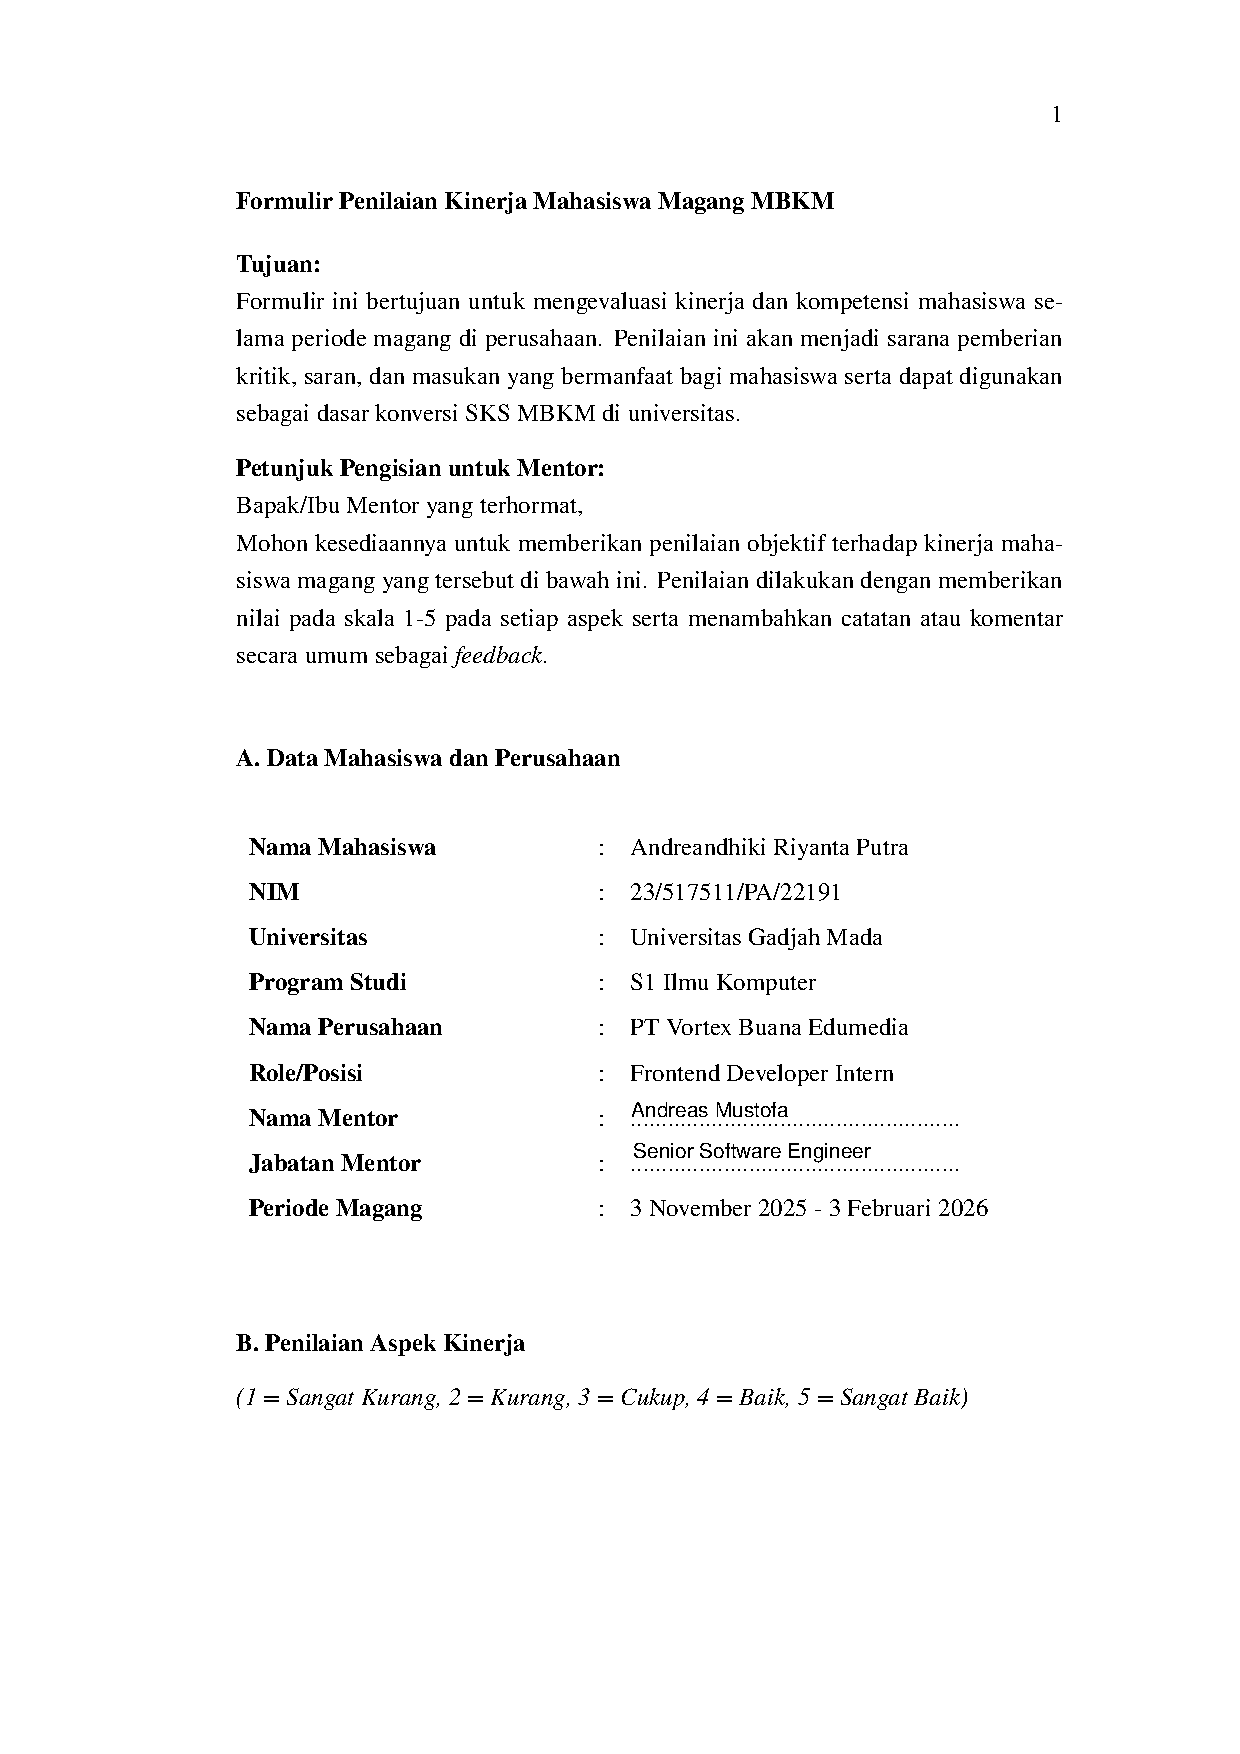
\includepdf[
	pages=-,
	frame=true,
	scale=0.8,
	pagecommand={\thispagestyle{fancy}}
]{assets/form_penilaian_mbkm_andreandhiki_riyanta_putra.pdf}


\chapter{Hasil dan Pembahasan}

\section{Pelaksanaan Kegiatan}
\lipsum[7]

\section{Pengujian Sistem}
Berikut adalah contoh pembuatan tabel profesional yang otomatis terdaftar di Daftar Tabel:

\begin{table}[htbp]
    \centering
    \caption{Hasil Pengujian Komponen}
    \label{tab:hasil_uji}
    \begin{tabular}{clc}
        \toprule
        \textbf{No} & \textbf{Skenario Uji} & \textbf{Status} \\
        \midrule
        1 & Rendering halaman utama & Berhasil \\
        2 & Pengambilan data API & Berhasil \\
        3 & Validasi form pengguna & Berhasil \\
        4 & Pengujian responsivitas UI & Berhasil \\
        \bottomrule
    \end{tabular}
\end{table}

Berdasarkan Tabel \ref{tab:hasil_uji}, seluruh fitur dasar berjalan tanpa hambatan.

\subsection{Implementasi Kode}
Potongan kode berikut menunjukkan implementasi dari komponen yang dibangun:

\begin{lstlisting}[language=JavaScript, caption={Komponen React Sederhana}, label={lst:react_code}]
import React, { useState } from 'react';

const UserProfile = () => {
    const [user, setUser] = useState('Dhiki');

    return (
        <div className="profile-container">
            <h1>Profil Pengguna</h1>
            <p>Selamat datang, {user}!</p>
        </div>
    );
};

export default UserProfile;
\end{lstlisting}

Listing \ref{lst:react_code} di atas merupakan contoh bagaimana state manajemen diterapkan.
\chapter{Penutup}

\section{Kesimpulan}
Berdasarkan hasil kegiatan magang dan pembahasan yang telah diuraikan pada bab-bab sebelumnya, dapat diambil kesimpulan sebagai berikut:
\begin{enumerate}
    \item \lipsum[8][1-3]
    \item \lipsum[8][4-6]
\end{enumerate}

\section{Saran}
\lipsum[9]

% --- BAGIAN AKHIR ---
\clearpage
\addcontentsline{toc}{chapter}{Daftar Pustaka}
\bibliographystyle{ieeetr}
\bibliography{src/bibliography/references}

% --- LAMPIRAN ---
\clearpage
\appendix % Mengubah format BAB menjadi Lampiran A, B, dst.
% Mengubah penamaan bab menjadi "Lampiran A", "Lampiran B", dst otomatis oleh LaTeX
\chapter{Tautan Repositori dan Dokumentasi Antarmuka}

Berikut adalah beberapa tautan dokumentasi, rancangan antarmuka (UI/UX), serta repositori kode yang dikerjakan selama masa magang untuk pengembangan sistem *frontend*:

\section*{1. Rancangan UI/UX (Figma)}
Seluruh rancangan antarmuka pengguna, komponen *design system*, dan purwarupa interaktif dapat diakses melalui tautan berikut: \\
\url{https://www.figma.com/file/dummy-link-rancangan-sistem}

\section*{2. Repositori Source Code (GitHub / GitLab)}
Repositori utama yang berisi implementasi kode menggunakan React/Next.js beserta dokumentasi teknisnya dapat diakses pada: \\
\url{https://github.com/organisasi-dummy/frontend-project-repo}

\section*{3. Dokumentasi Tampilan Website (Live Demo)}
Sistem yang telah di-*deploy* ke *environment staging* untuk keperluan pengujian dapat diakses melalui: \\
\url{https://staging.dummy-project.com}

\vspace{1cm}

\chapter{Dokumentasi Kegiatan Lapangan}

\begin{figure}[htbp]
    \centering
    % Placeholder untuk foto kegiatan, ganti dengan \includegraphics[width=0.8\textwidth]{foto-kegiatan.jpg}
    \rule{12cm}{7cm}
    \caption{Tangkapan layar hasil implementasi komponen UI pada sprint ke-3}
    \label{fig:lampiran_kegiatan1}
\end{figure}

\begin{figure}[htbp]
    \centering
    \rule{12cm}{7cm}
    \caption{Diskusi penyesuaian integrasi API bersama tim *Backend*}
    \label{fig:lampiran_kegiatan2}
\end{figure}

\chapter{Lampiran LOA}

\section*{1. Letter of Acceptance}
\begin{figure}[htbp]
    \centering
    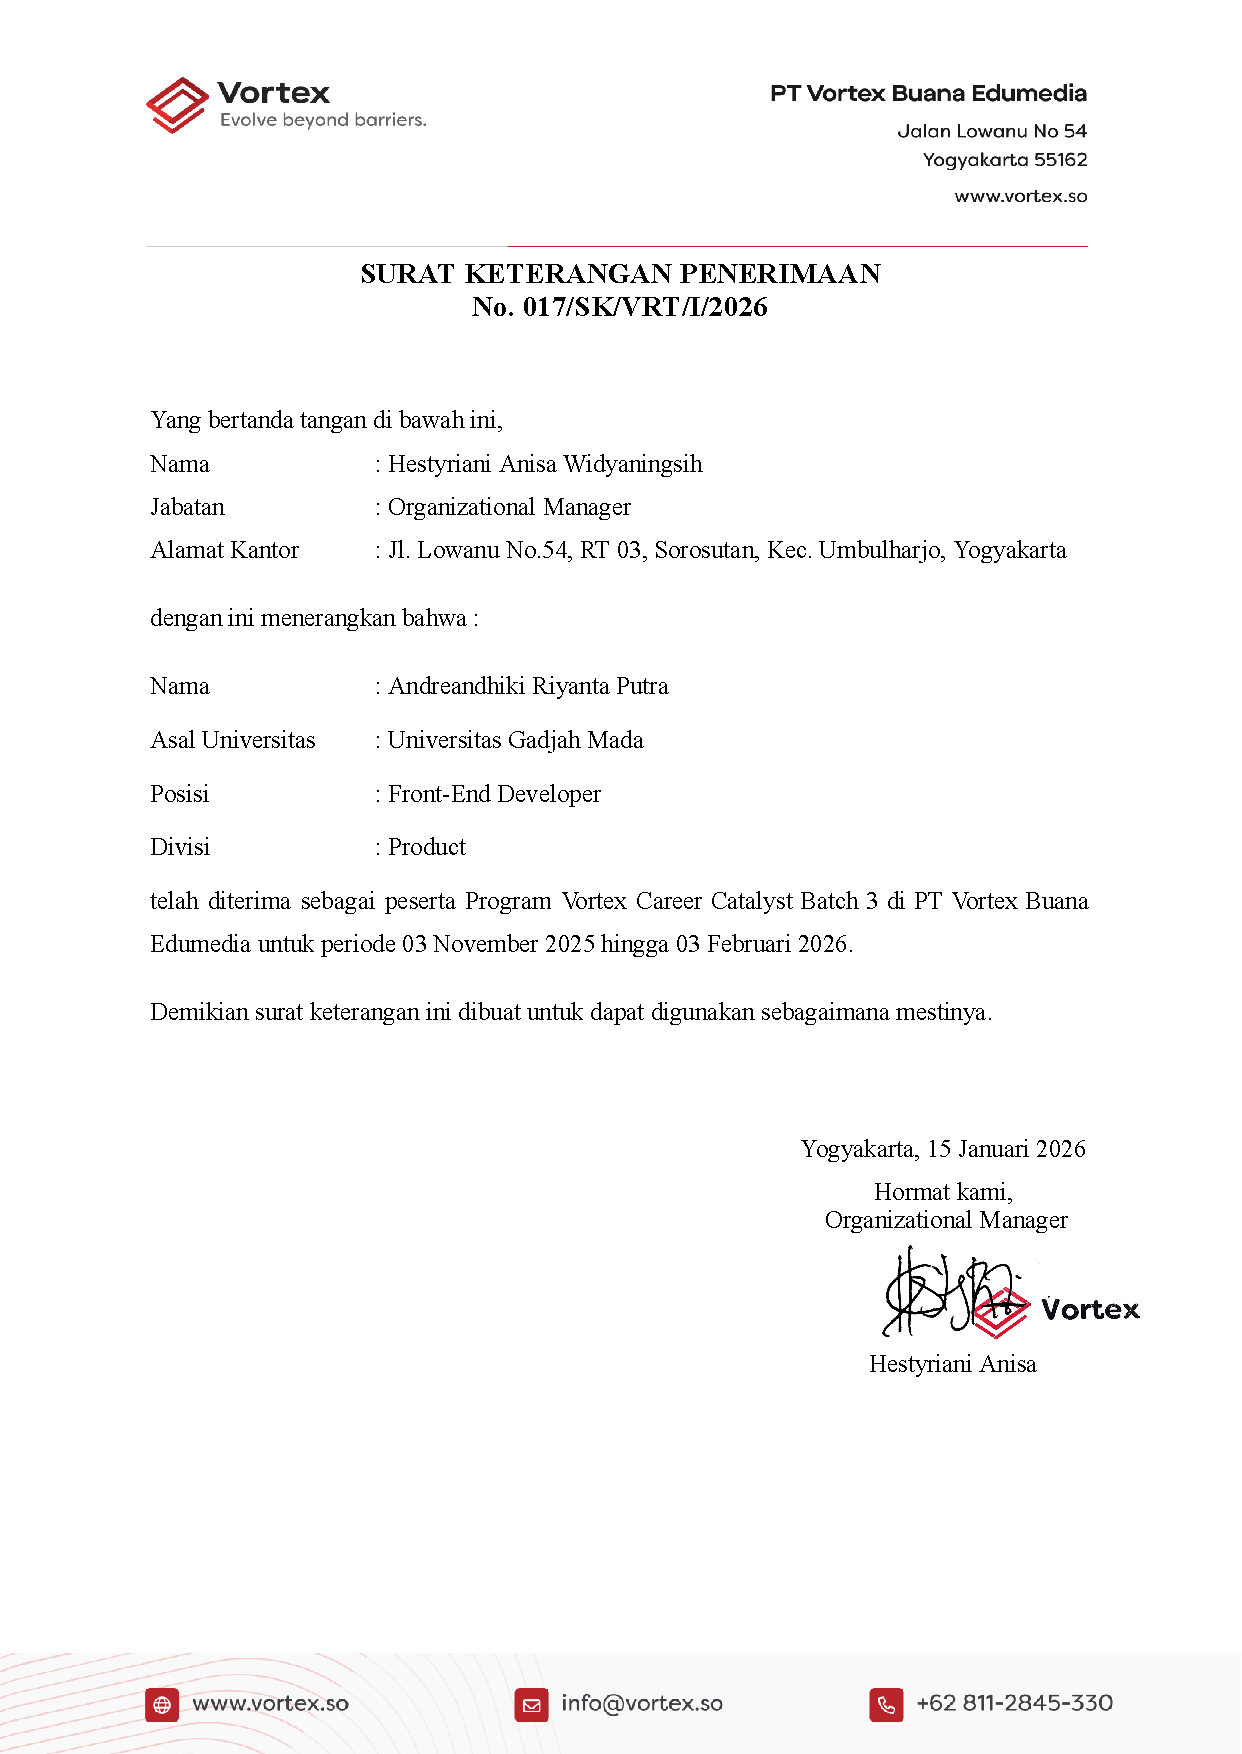
\includegraphics[width=\textwidth,height=0.72\textheight,keepaspectratio,page=1]{assets/LOA.pdf}
    \caption{Letter of Acceptance (halaman pertama)}
    \label{fig:lampiran_loa}
\end{figure}

\end{document}
